% !TEX program = lualatex
\documentclass{antiquebook}

%--------------------------------------
\usepackage{graphicx, float, setspace, csquotes}
\usepackage[object=vectorian]{pgfornament} %%  http://altermundus.com/pages/tkz/ornament/index.html
\usepackage{pgfplots}
\pgfplotsset{width=10cm,compat=1.18}
\renewcommand{\baselinestretch}{1.4} 
\newcommand{\sectionline}{%
  \noindent
  \begin{center}
  {\color{black}
    \resizebox{0.5\linewidth}{1ex}
    {{%
    {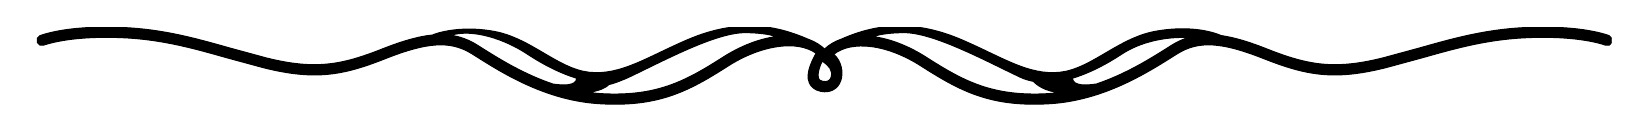
\begin{tikzpicture}
    \node  (C) at (0,0) {};
    \node (D) at (20,0) {};
    \path (C) to [ornament=85] (D);
    \end{tikzpicture}}}}}%
    \end{center}
  }
%--------------------------------------

\author{Pranav Upreti}
\title{An Engineering Design Handbook}
\date{}

%\input{glossary.tex}

% goal: around 700 max words

\begin{document}
	\frontmatter
	\maketitle
		\hspace{0pt}
		\vfill
		\begin{center}
			Copyright © 2025 by Pranav Upreti

			All rights reserved.

			No portion of this book may be reproduced in any form without written permission from the publisher or author, except as permitted by Canadian copyright law.

			Illustrations by Pranav Upreti 
		\end{center}
		\newpage
		\hspace{0pt}
		\vfill
		\begin{center}
			\textit{This handbook is dedicated to my best friend Milo}
			\begin{figure}[H]
				\centering
				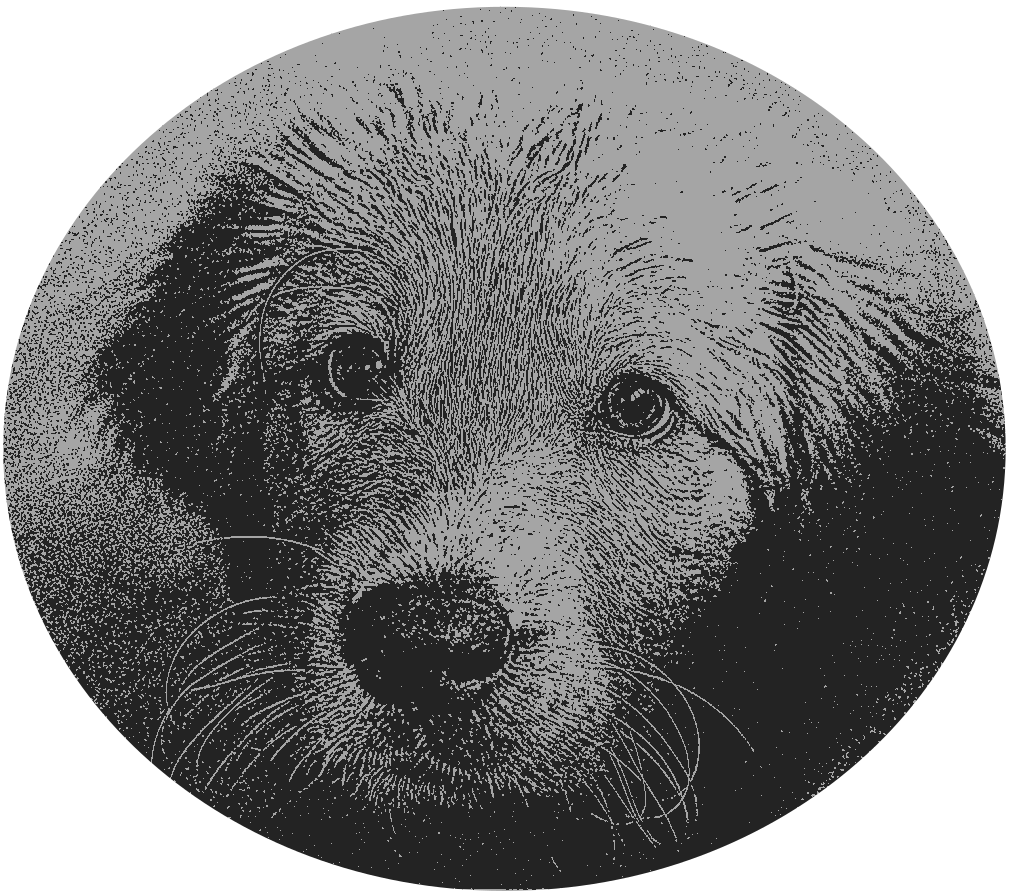
\includegraphics[scale=0.5]{MiloOfficial.png}
			\end{figure}
		\end{center}
		\vfill
	\chapter*{Preface}
	Engineering design is not something that can be taught traditionally through lectures and exams. It is instead (i) informed through experience and (ii) observing others approach engineering. This handbook aims to aid with the latter, by providing an overview and reflection on my engineering design approach. 

	You'll notice that I convey my experiences with in an old and battered engineering handbook style. It suggests that my vision for engineering design is rooted in ideas formulated by those before me. It also hints that some of my ideas are outdated, and will be subject to revision. 

	This style was emulated through the awesome typesetting language \LaTeX{}. I'd like to extend my gratitude to Masum Billal who created \texttt{antiquebook}, which is the class I used to create this handbook. 
	
	I hope you enjoy reading and maybe even learn a thing or two :D. \\[30pt]

	\noindent Regards, \\
	Pranav Upreti 


	\newpage
	\tableofcontents
	\newpage
	\mainmatter
	\pagestyle{fancy}
	\chapter{A Design First Approach to Engineering Design}
	\section{What is Engineering Design?}
	Engineering design is a combination of ``engineering'' and ``design''. \\[6pt]
	%definition: engineering
		\noindent\fbox{%
		\parbox{\textwidth}{%
			\textsc{Definition: } Engineering \\
			Engineering is the use of theoretical and experiential knowledge (i.e. science) to \textit{create} something of practical use. That is, create something that conforms to a set of requirements derived from an opportunity. This practicality element is what separates a scientist from an engineer. \\
		}
		} \\[6pt]
		\noindent\fbox{%
		\parbox{\textwidth}{%
			\textsc{Definition: } Design \\
			Design is how a stakeholder interacts with an object. It is related to how the object is used (i.e. if it is held, does it fit in your hand? if it is worn, is it comfortable? is it nice to look at?). Design is subjective compared to engineering, because questions like ``is my design nice to look at'' depend on the stakeholder. 
			As an additional constraint, I propose a ``good''/``better'' design is easily forgotten. For instance, consider the design of a phone. If the phone is comfortable, light, and nice to look at, you forget about it. But if the phone is spikey, it pokes and hurts you every time you hold it. You cannot forget about that design since it hurts, so it has a \textit{comparatively} ``bad'' design.  
			}% 
		}\\[6pt]


		When we combine ``engineering'' with ``design'', we get that engineering design is about identifying an opportunity, developing a set of requirements, creating a solution to the opportunity, and ensuring that the solution is easy for the stakeholder to interact with. 

		\sectionline

		Naturally, the question becomes: which contributes more to the engineering design: ``engineering'' or ``design''? The prudent or perhaps lazy answer is that it depends on an opportunity. I disagree; ``design'' is nearly always more important than the ``engineering''\footnote{This may change as I gain experience}. 

		Remember that the goal of any engineering design is to meet the requirements dictated by stakeholders. Suppose there are multiple solutions to an opportunity that work just as well. The stakeholder will choose the solution that has the best design\footnote{Remember we qualified ``good'' designs as being the easiest to interact it with. And by interact with, we include its appearance, feel in hand, ease of use, weight, and more depending on the nature of the solution}.

		I argue that the engineering design process should start by exploring the \textit{``best'' design}. That is, identify the form of the solution that is easy and pleasant for stakeholders to interact with. Importantly, if the solution is tangible, care should only be given to meet requirements pertaining to the form of the solution (i.e. dimensions, weight, colour, etc.). Then, the engineer figures out how to make said design meet all other stakeholder requirements. This approach fosters creativity, since your solution space is only constrained by a subset of requirements. It may be difficult to meet all other requirements, but that is what makes engineering so fun. If you do not think it is possible to meet the entire set of requirements with a design-first approach, you are not trying hard enough. 

	\chapter{Two Key Learnings}
	My version of engineer design is the culmination of \textbf{two key learnings}: (i) every detail counts and (ii) the importance of iterative design. 
		\section{Every Detail Counts}
		One of the key values that is reflected in my engineering design process is a (sometimes excessive) attention to detail. My dad explained why this is important growing up with a story of a Nobel Laureate, after noticing me sloppily putting a jacket on a hanger.
		\begin{displayquote}
			\it 
			Prisoners during British colonization were forced to fold envelopes, so they usually did a sloppy job. One prisoner folded everything immaculately; when asked why, he simply said doing quality work, even of menial tasks, is a habit. 
		\end{displayquote}
		This stuck with me. The difference between a good solution and a great solution is the attention given to small details. 
		
		A disadvantage to this value is that I do not feel most people want to spend the same amount of time I do on these little details. This has led me reluctant to working in teams, even though engineering is very much a collaborative effort; I felt unsatisfied coming out of group efforts. 

		This is undoubtedly something I intend on being more comfortable with, because I do value the brainpower boost when working in a team. I have just developed a false pretense that I can deliver higher quality work working alone because I can control every tiny detail. I have started improving by joining design teams this semester!
		\section{Learning 2: Iterative Design}
		My impression of engineering design growing up was that engineers were geniuses who could solve any problem. This is actually why I chose engineering; I want to be skilled enough to help anyone with any problem. Although I am hopefully approaching being able to learn thermonuclear astrophysics in a night\footnote{This is a reference to Tony Stark a.k.a. Iron Man, who is the coolest fictional engineer there is.} (if I can get off my phone), I still rely on iterative design.

		My favourite analogy on iterative design comes from YouTuber Mark Rober. Imagine the design space is a 3D contour plot; the optimal solution is the highest peak on the plot. The only way to get this optimal solution is to start somewhere arbitrary, and as you iterate your design, you move up to a peak. This process takes time, because the solution space is large. 

		\begin{figure}[H]
		\begin{center}
		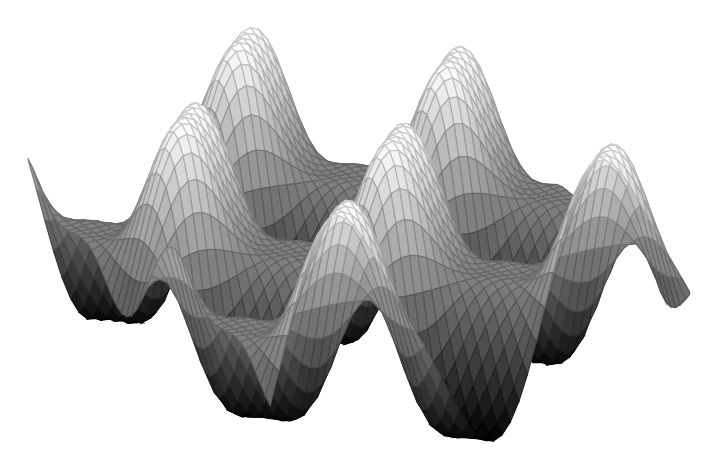
\begin{tikzpicture}
			\begin{axis}[
				view={60}{30},
				axis lines=none,
				colormap/blackwhite,
			]
			\addplot3[
				surf,
				samples=50,
				domain=-5:5,
				y domain=-5:5
			]
			{sin(deg(x)) * cos(deg(y)) + 0.3 * sin(deg(2*x)) * sin(deg(2*y))};
			\end{axis}
		\end{tikzpicture}
		\end{center}
		\caption{A 3D contour plot}
		\end{figure}
		Through iterative design, I have realized I value \textbf{dedication}, since I want to iterate a design to perfection.

	\chapter{An Exercise in Engineering Design}
	I'd like to conclude with an annotated photo journey through an engineering design which demonstrates my \textbf{design-first} approach. \\[12pt]
	\textit{The Opportunity:} A light up sword as a birthday present for my mom.
	\begin{figure}[H]
		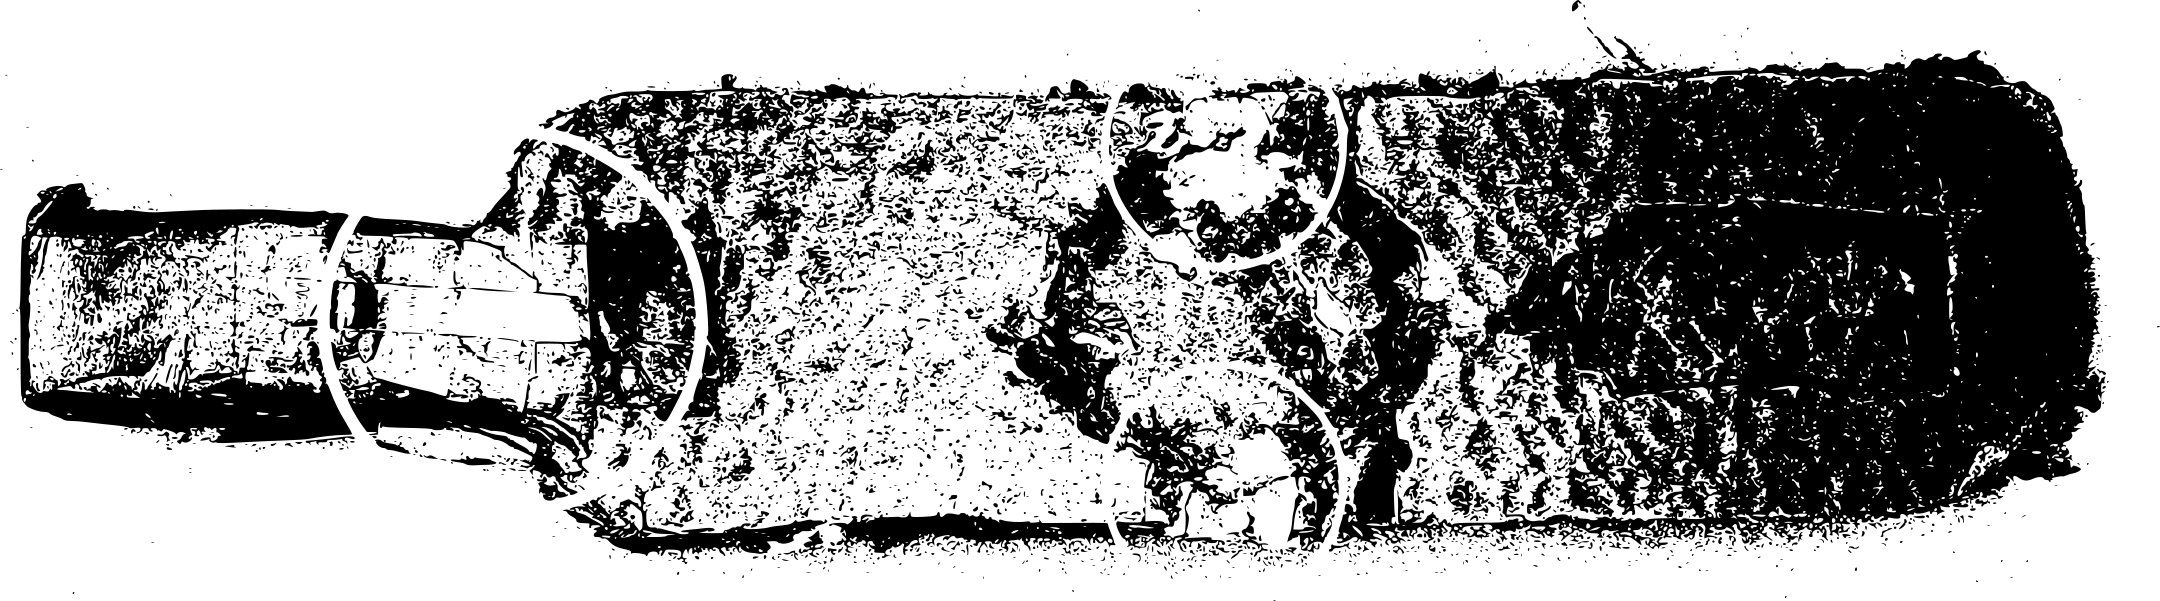
\includegraphics[width=\linewidth]{swordv1.png}
		\caption{\textbf{V1}\quad A design-first approach: I decided how the sword should look and feel. All electronics were shoved into the little space in the design. This was not structurally sound, and it broke EVEN with duct tape and glue.}
	\end{figure}
	\begin{figure}[H]
		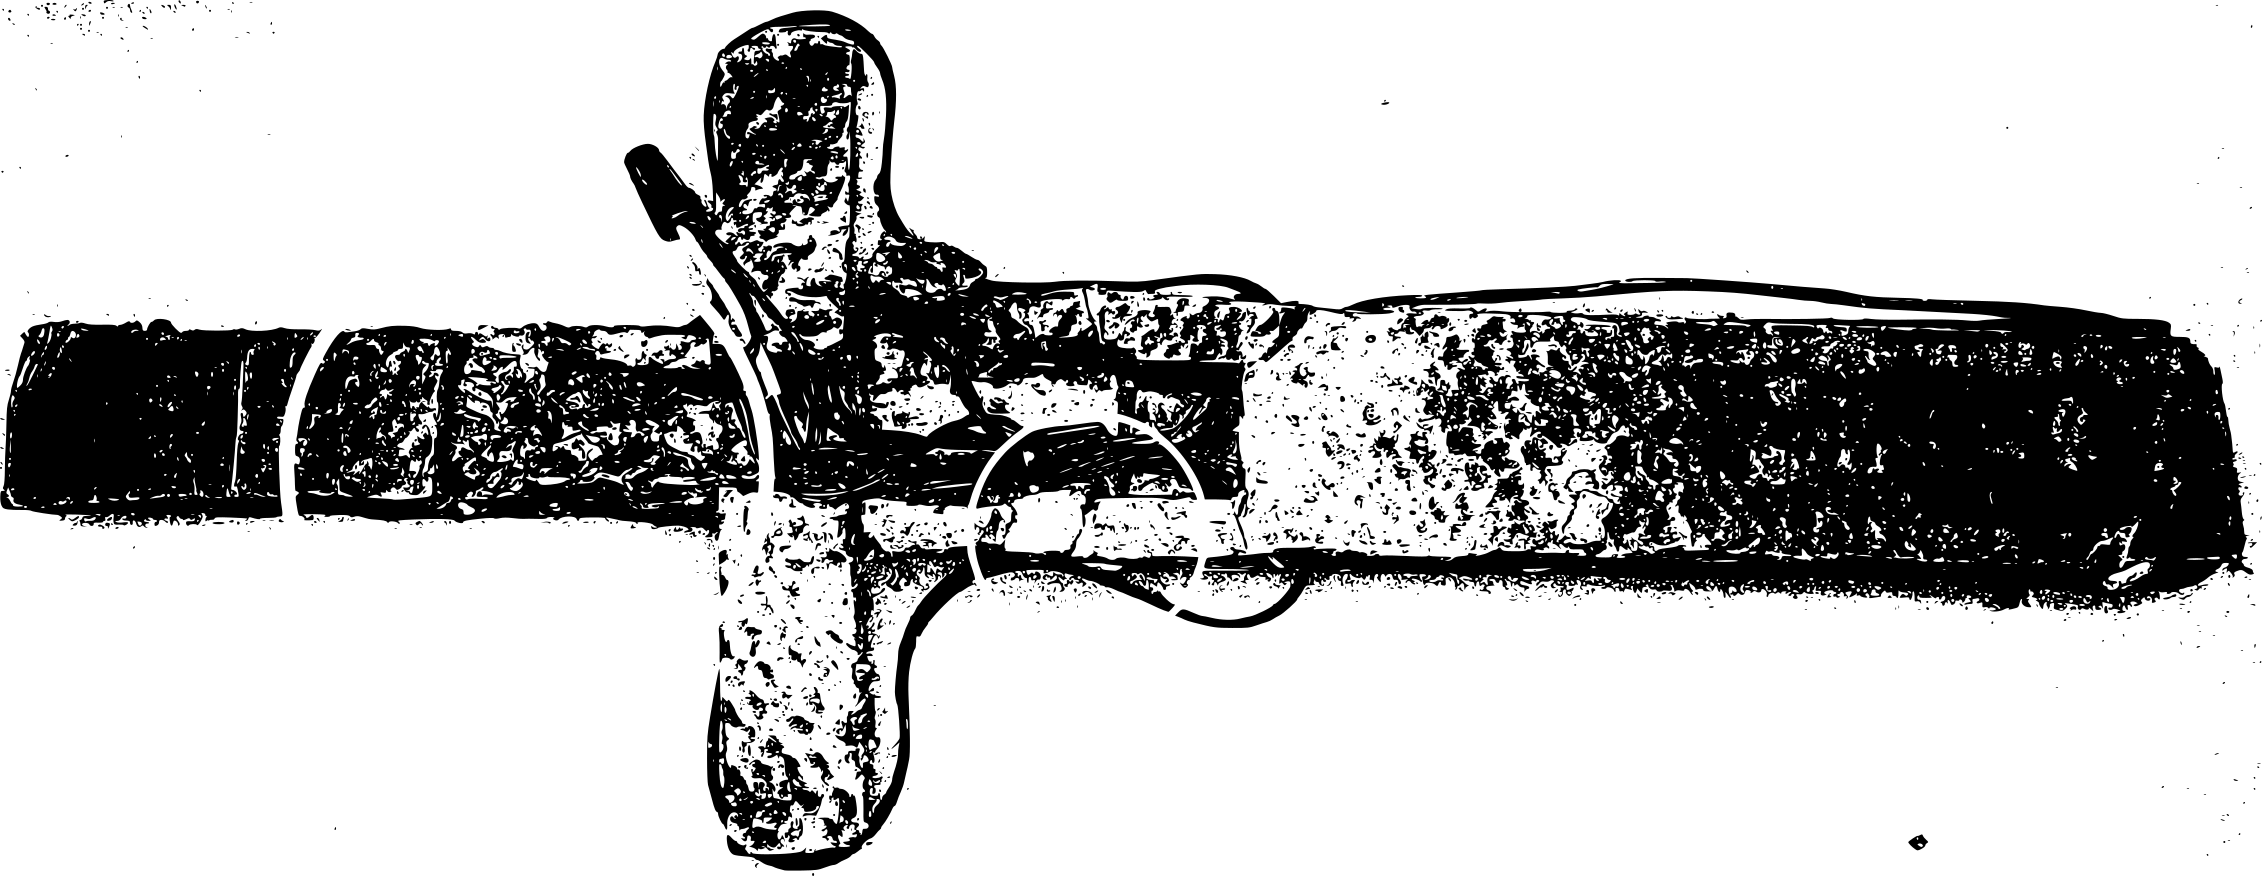
\includegraphics[width=\linewidth]{swordv2.png}
		\caption{\textbf{V2}\quad V2 performed similarly. I made tweaks to the styling, and still shoved the electronics in. Still broke too easily.}
	\end{figure}
	\begin{figure}[H]
		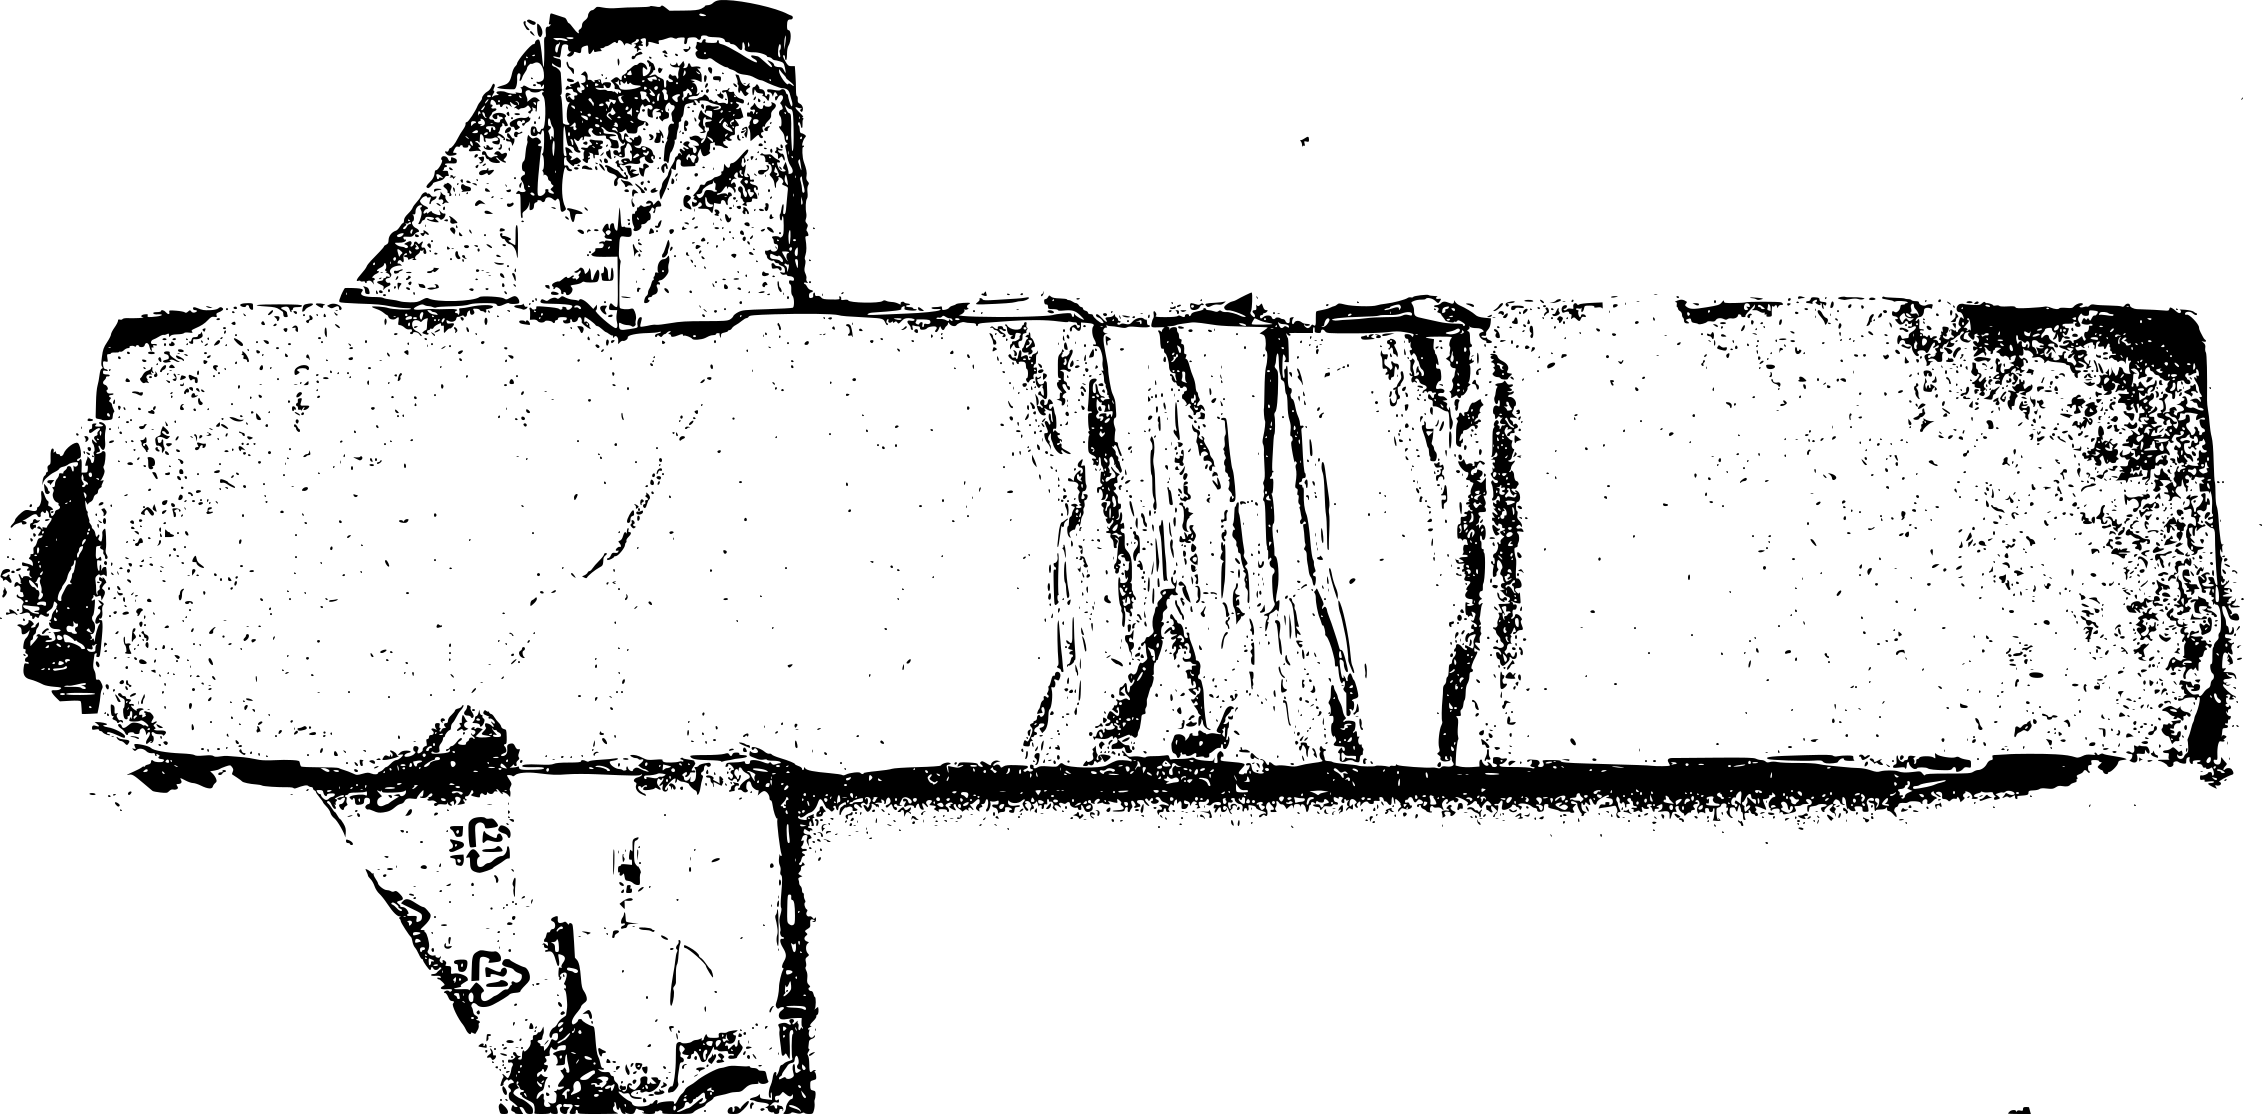
\includegraphics[width=\linewidth]{swordv3.png}
		\caption{\textbf{V3} \quad For V3, I tried designing the sword to fit the electronics, rather than the electronics fitting into a design I thought was ``good'' (it looked and felt nice to hold). Although it was stronger, it looked ugly. This reinforced that I should focus engineering the electronics to fit into a design I liked.}
	\end{figure}
	\begin{figure}[H]
		\scalebox{-1}[1]{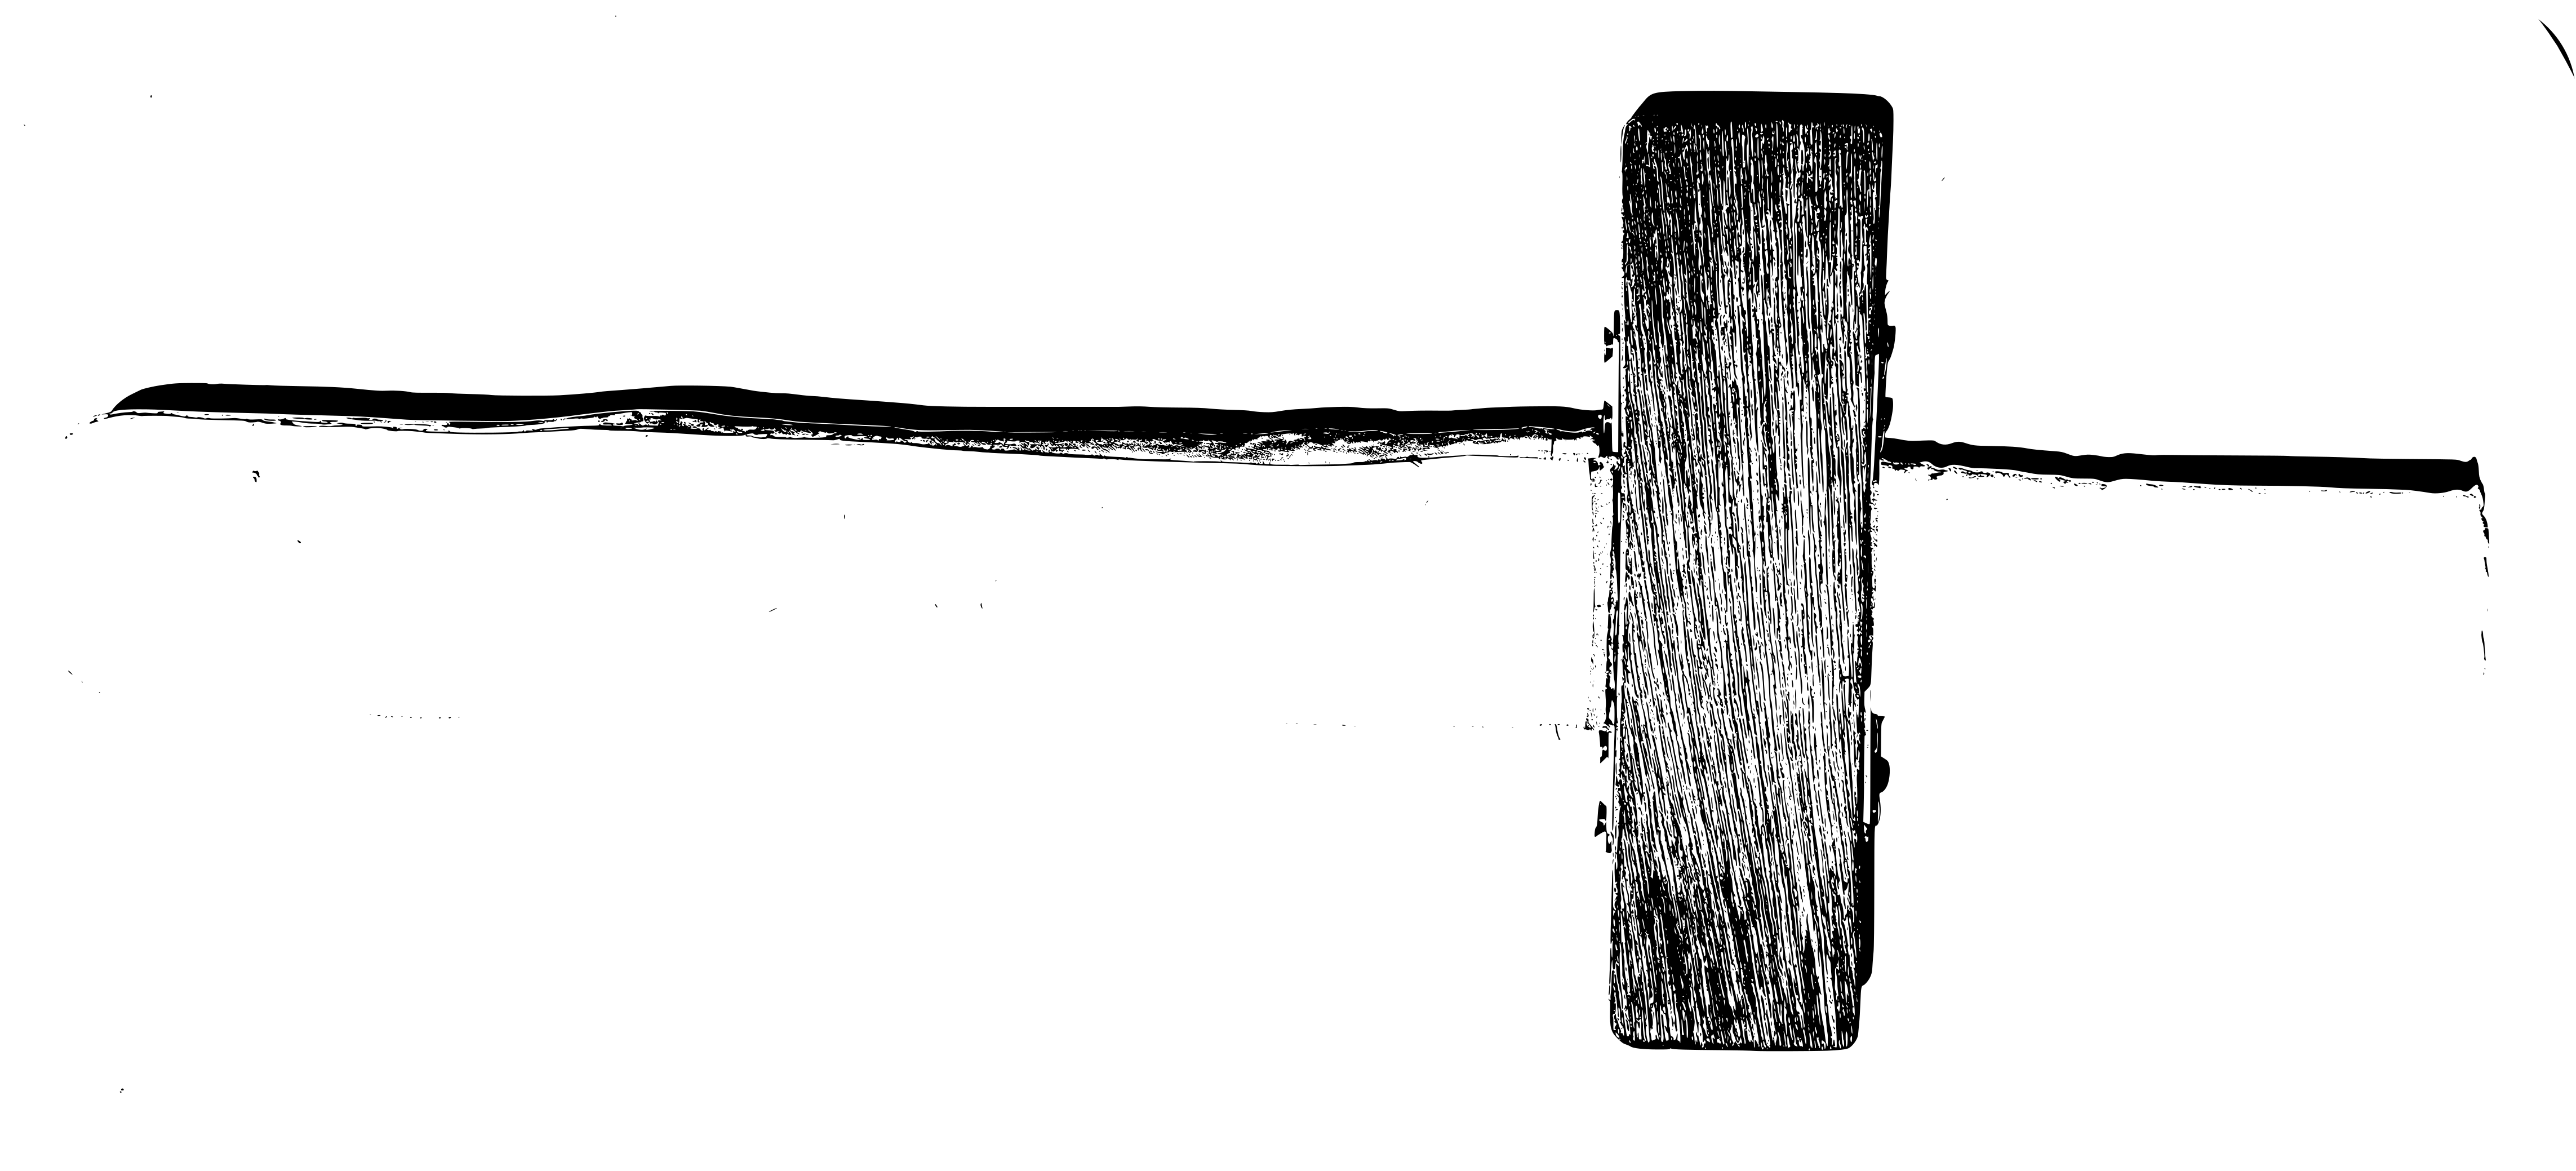
\includegraphics[width=\linewidth]{swordv4.png}}
		\caption{\textbf{V4} \quad V4 went back to looking like V2. I changed the material to wood instead of cardboard, so it was structurally sound. By picking a design and sticking with it, I was able to figure out how to incorporate other requirements (i.e. required electronics components) \textit{into} my chosen design. }
	\end{figure}

	This engineering design project took 6 months to complete, with 4 iterations to create a product I was happy with. I was more happy with how my mom liked the present. This reinforced my reason for studying engineering: if I can help people, perhaps by spreading joy or fixing things, that makes everything I am learning worthwhile.
	
	This was my first long-term engineering project, back in grade 8, so I am surprised my design-first approach has been so consistent throughout the years. As a closing remark, I expect my engineering design process to change in the coming years. Future projects and opportunities will require more thought and time; I may very well pivot my engineering design process to incorporate new values. The future will challenge and force me to grow, which is something I am excited for.



	
\end{document}